\chapter{Development components}
\label{ch:development-components}

\section{Development workflow}
\label{sec:development-workflow}

\begin{figure}
\centering
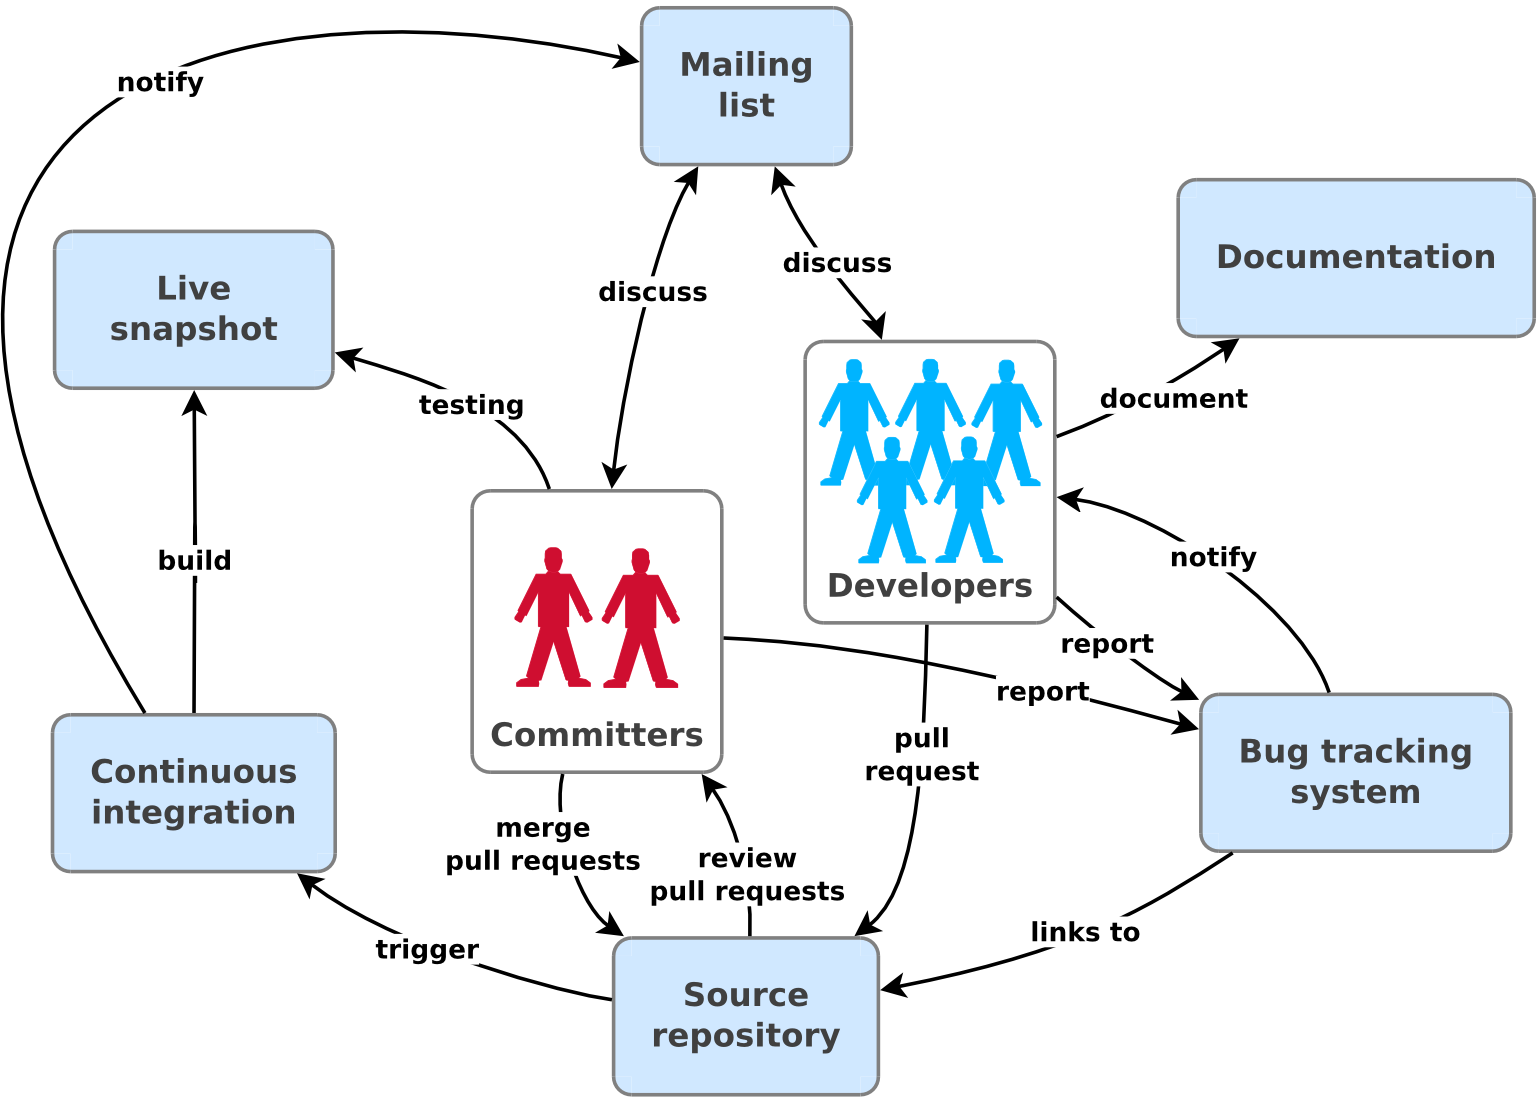
\includegraphics[width=0.67\textwidth]{images/development-workflow.png}
\caption{Development workflow with all tools}
\label{fig:development-workflow}
\end{figure}

\section{Details}
\label{sec:details}

The Figure~\ref{fig:development-workflow} illustrates the global development workflow.
In this workflow, there is two different kind of actors (developers and integrators) which
interact with different kind of tools.
We will now give more details on these tools and how they will be used by the actors.

\subsection{Mailing list}
\label{sec:mailing-list}

An email mailing list will be available for general decision making about the platform,
the goal being to keep records of discussions and choices about developments or architecture design.

\subsection{Source repository}
\label{sec:source-repository}

A distributed source code repository will be provided for storing the source code or binaries
needed for building the \learnpad platform.

Developers will propose new functionality or bug fixing using \emph{pull requests}
\footnote{A pull request is a method of submitting contributions to a software project.
It contains the \emph{patch} representing changes to be made and creates a central place
for those changes to be reviewed and discussed}
which integrators will have the duty to review. An integrator may and accept the
\emph{pull request}, request changes or further information or in an extreme case,
close it pending further discussion.

Despite having direct access to the shared repository, an integrator who is also a developer should
make sure to use \emph{pull requests} for integrating their own functionality so as to allow for
discussion with other integrators and developers and to keep record of the contribution.

All developers should adopt the \emph{check in early and often} development methodology.
Code in development is not expected to be bug-free but great importance is placed on collaboration
and working in the open. In a fast-changing collaborative software development project, frequent
pull requests help everybody. They help the developer making them because he is able to avoid
rewriting code to cope with changes in other elements of the system and they also help other
developers who are able to see and adapt to changes in this developer's component.

\subsection{Documentation}
\label{sec:documentation}

Documentation will be able to be written accompanying the source code in the repository or it
may be places on a provided wiki as long as relevant documents are referenced from the source
repository.

\subsection{Bug tracking system}
\label{sec:bug tracking-system}

All participants will be responsible for discovering and diagnosing of bugs. Bugs, feature
requests and other to-do items shall be reported to a provided bug tracking system where others
will be able to keep track of issues which need to be addressed. Email notifications of new
issues will be sent to integrators and updates of an issue will be sent to those who participate in
(EG: comment on) the issue.
